\chapter{Clinical validation}
 
\section{Organ transplantation}
 
In organ transplant recipients, the ratio of recipient genomic DNA to graft-derived donor DNA, distinguished by SNPs that are specific to the recipient or the donor, provides a measure of the number of graft cells that are dying and releasing their DNA into the blood. In a pilot study of heart transplant recipients, episodes of acute cellular organ rejection were marked by increases in the proportion of donor-derived DNA in the blood. Advantages of this approach over traditional periodic biopsies of the graft tissue are that it is less invasive, may be less affected by sampling errors if lymphocytic infiltrates or regions of cell \cite{Snyder:2011gd}.
   
We first applied the infectome pipeline to existing cell-free DNA samples banked and processed by the Quake lab. These samples were largely from organ transplant recipients because rejection can be monitored by quantifying cell-free donor-specific DNA in the transplant recipient?s plasma via shotgun sequencing (?genome transplant dynamics?, GTD). By using single nucleotide polymorphisms (SNP) to discriminate between donor and recipient DNA molecules, GTD provides a non-invasive yet direct measure of graft damage. In this cohort, immunosuppressive therapies significantly reduce the risk of graft rejection, but increase the susceptibility of recipients to infections. Together with allograft rejection, infectious complications remain one of the most important causes of morbidity and mortality after lung transplantation, with cytomegalovirus infections (CMV) posing the most significant known threat. 

With this in mind, we explored whether cfdDNA levels correlate with clinical indicators of infection. Infectious pathogens are identified by simultaneously identifying non-human cfDNA sequences and comparing them to known genomic databases of bacterial, viral and fungal pathogens. To study the relationship between infection and graft damage, we collected over 35000 clinical measurements of specific infections performed on 14 specimen types for the lung transplant cohort. We first quantified reads that map to the CMV genome for each sample and observed increased CMV abundance in samples that were clinically positive for infection, resulting in an AUC of $0.91$ Figure ~\ref{fig:Fig9}). This data indicates that CMV surveillance can be performed in parallel with rejection monitoring using the same sequence data and led us to examine whether other viral infections could be similarly monitored.

\begin{figure*}
\center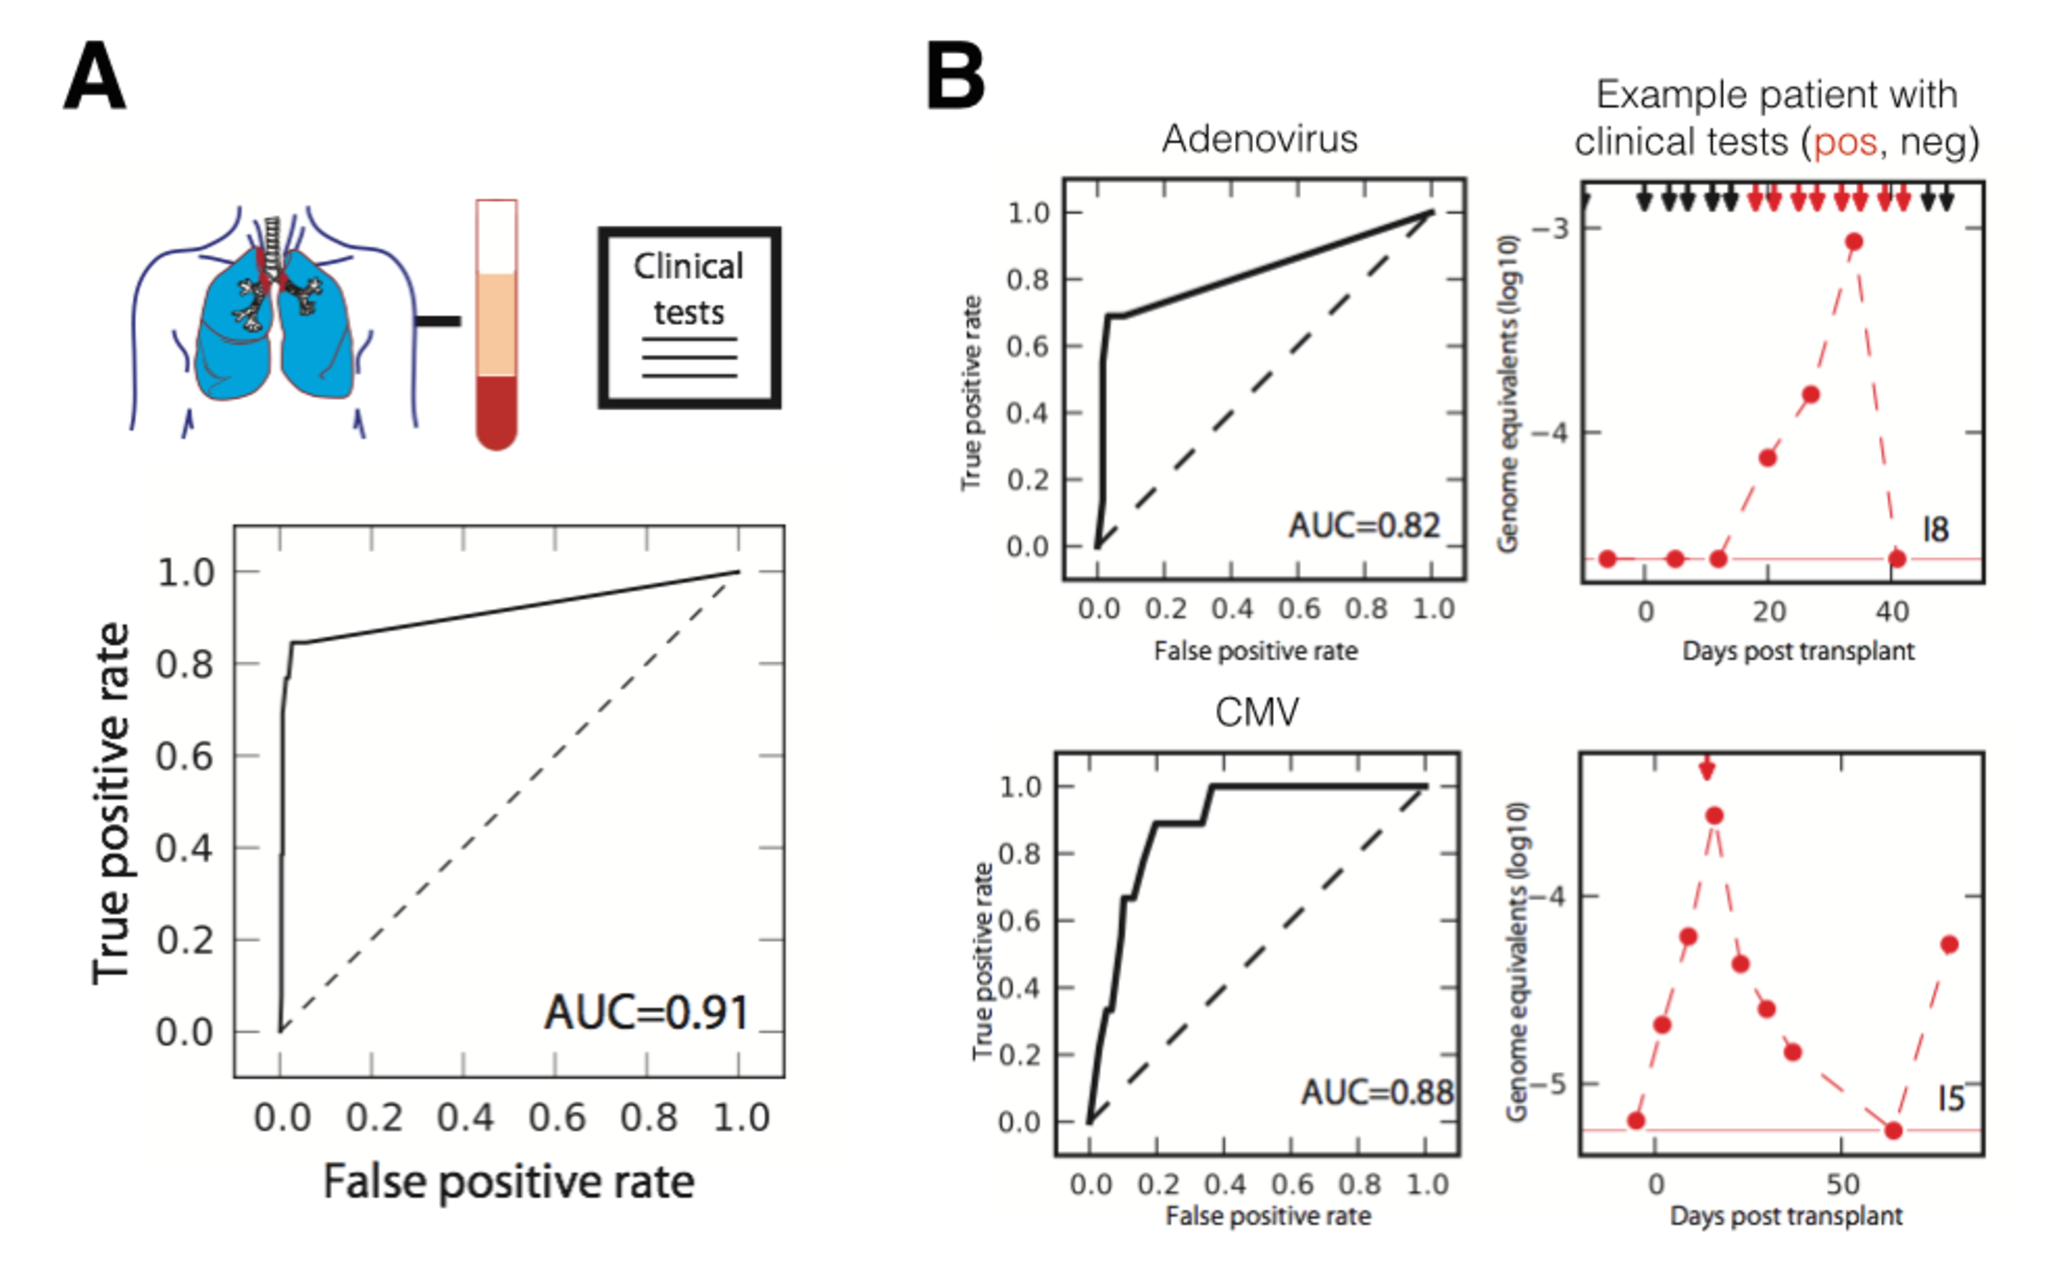
\includegraphics[width=150mm,scale=0.5]{Figures/Fig9}
\caption{Clinical correlations on viruses}
\label{fig:Fig9}
\end{figure*}

We next performed a similar analysis on a pediatric bone marrow cohort. Like lung, clinical testing for CMV was common. Because of the elevated risk in the pediatric cases, this cohort includes regular screens for additional viruses. For example, Adenovirus is a community-acquired respiratory infection that can cause graft loss in transplant recipients and poses a particularly high risk for paediatric patients. The correlation between infection-derived cfDNA and positive clinical tests for viruses are evident in timeseries data, at elevation in signal is observed when positive clinical test results are recorded (Figure ~\ref{fig:Fig9}), and is further captured at cohort-level with ROC curves that have favorable AUC values of $0.82$ and $0.88$ for Adenovirus and CMV, respectively. 

Collectively, the favorable performance on viruses is reasonable. Existing clinical test are performed on blood using molecular diagnostics, such as qPCR. With this in mind, the observed performance of NGS on cell-free DNA is not surprising. However, it is worth noting that the performance is quite encouraging considering the fact that these samples are not enriched for non-human signal. Indeed, infection-derived cell-free DNA is sparse in the sequencing libraries and, therefore, the favorable performance should only be expected to improve as greater depth is reached through enrichment strategies.

\begin{figure*}
\center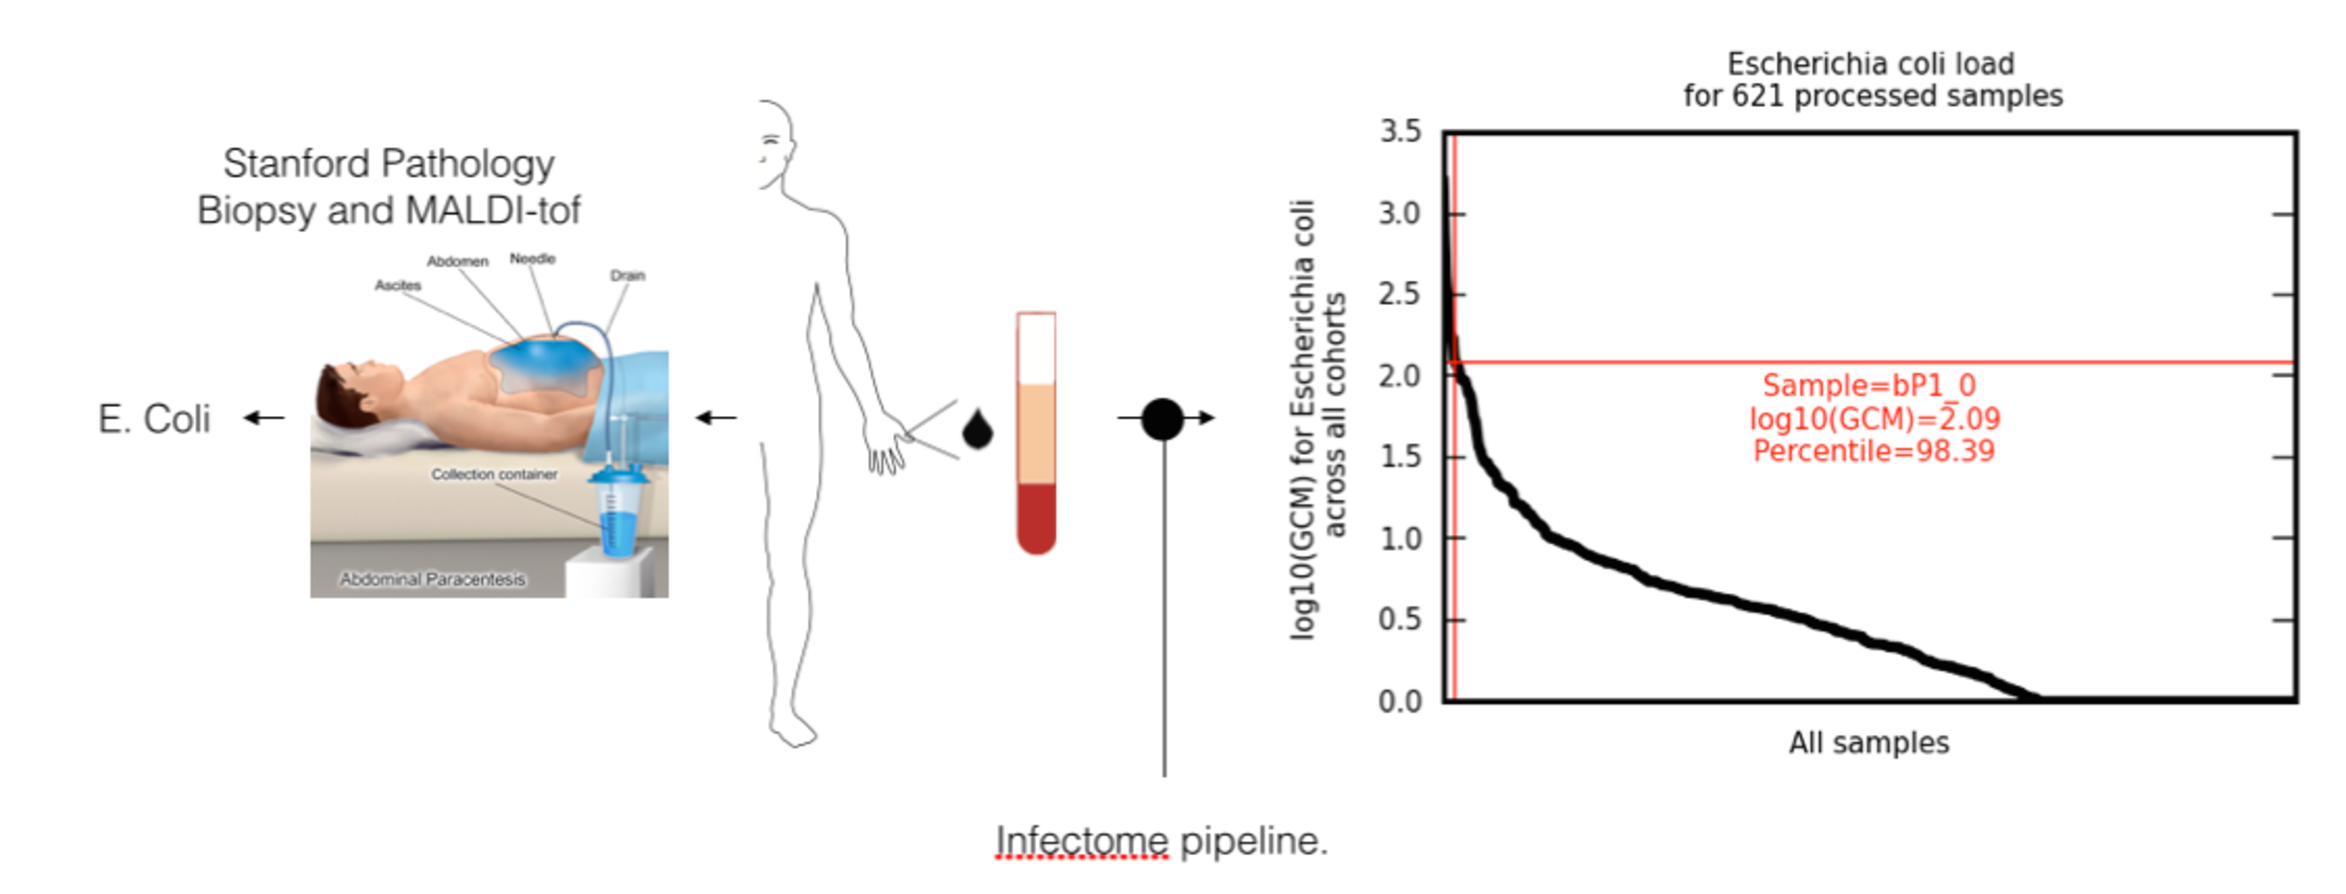
\includegraphics[width=150mm,scale=0.5]{Figures/Fig10}
\caption{Clinical correlations with deep tissue sampling}
\label{fig:Fig10}
\end{figure*}

\section{Deep tissues}

We next examined the ability to resolve deep-tissue infections using blood as the sampled medium. This would be particularly appealing, because invasive biopsies to test for infection can be problematic for patients with compromised heath and can introduce risk. To examine this, we compared shotgun sequencing of blood biopsy sampled from a gastrointestinal abcess tested using MALDI-tof. The biopsy results (positive for E. Coli) agree with the cfDNA sampling, which shows that this patient have a very higher percentile E. coli measurement relative all all samples processed (Figure ~\ref{fig:Fig10}).

\section{Untested infections}

Considering the favorable results on both vises as well as bacteria, we further examined the merits of hypothesis-free screening by examine data for the lung transplant cohort. We identified well characterized pathogenic and onco-viruses as well as commensal torque teno viruses (TTVs, alphatorquevirus genus) in that data, is consistent with previous observations of a link between immunosuppression and TTV abundance. The frequency of clinical testing for these viruses varied considerably, with frequent surveillance of CMV (Human Herpes Virus 5, HHV-5) relative to other pathogens (Figure ~\ref{fig:Fig11}). 

\begin{figure*}
\center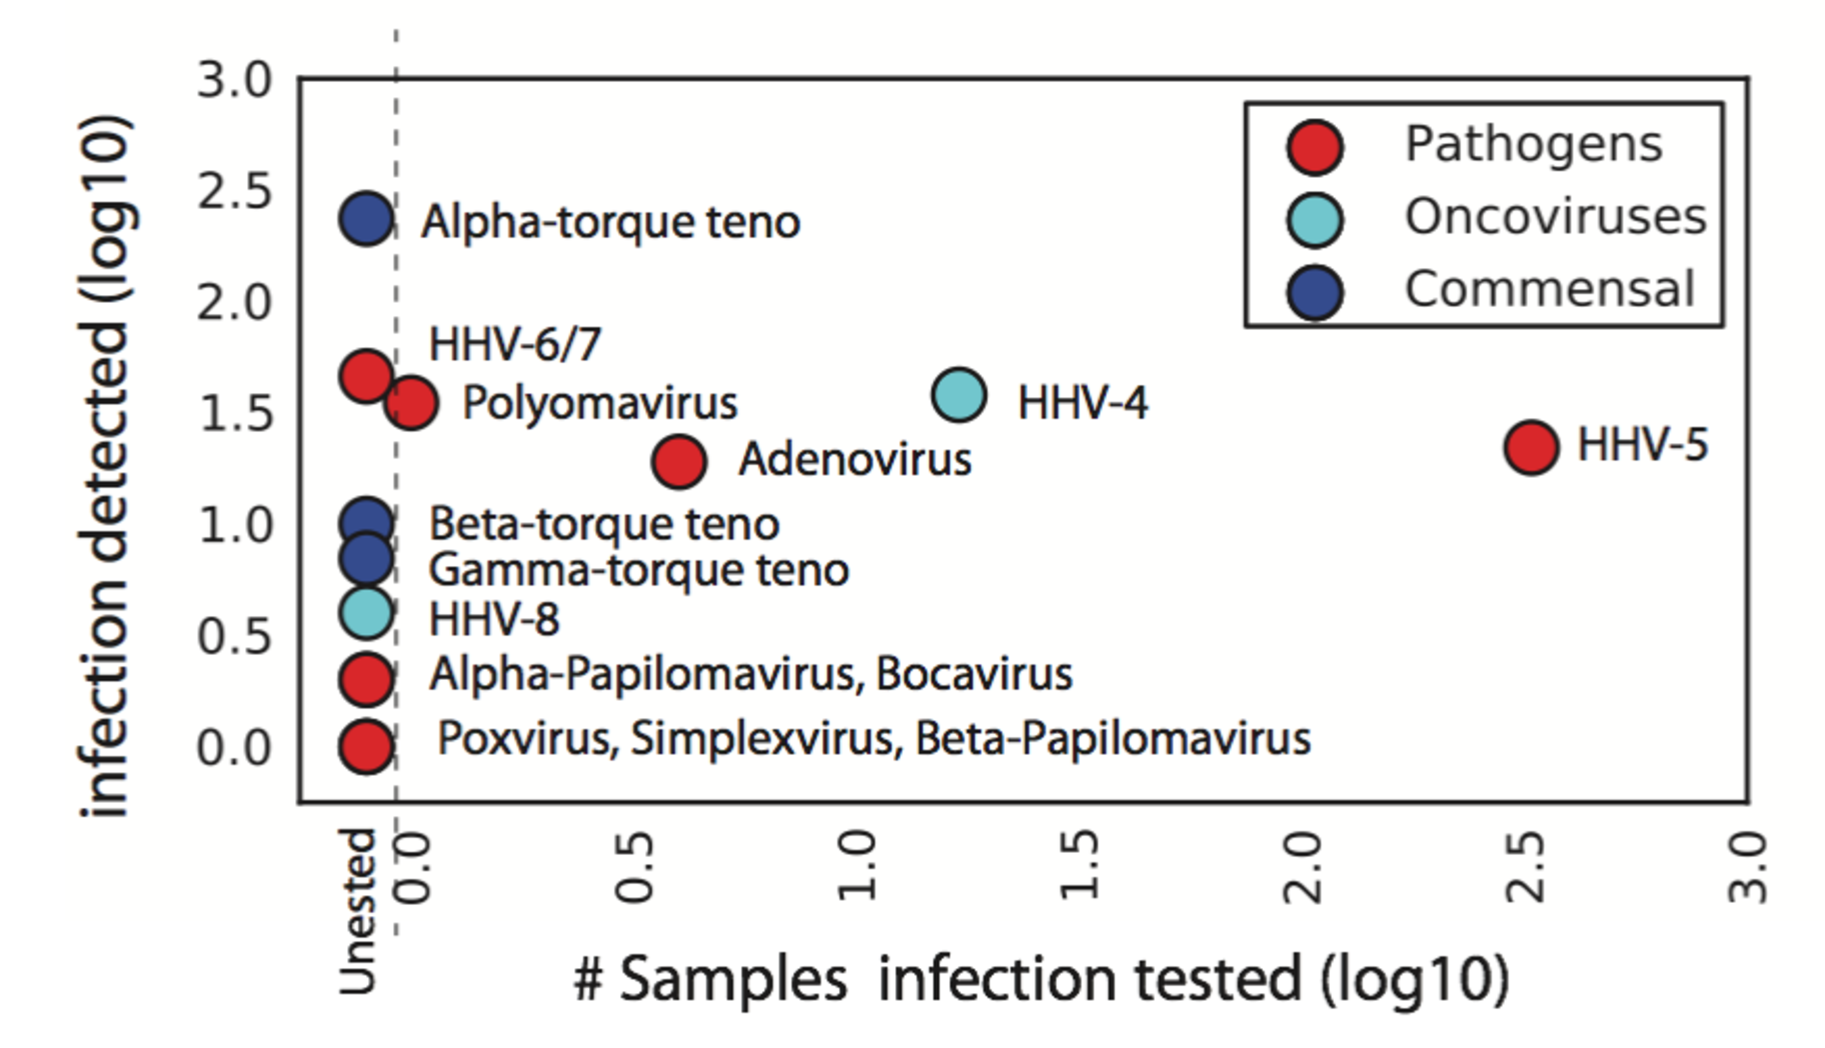
\includegraphics[width=150mm,scale=0.5]{Figures/Fig11}
\caption{Clinical correlations on viruses}
\label{fig:Fig11}
\end{figure*}

We evaluated the incidence of infection (number of samples in which a given virus is detected via sequencing) relative to the clinical screening frequency. Although CMV was screened for most frequently (335 samples), its incidence as determined by sequencing (detected in 22 samples) was similar to that of other pathogens that were not routinely screened, including adenovirus and polyomavirus (clinically tested on four occasions and one occasion, respectively). We further showed that hypothesis-free infection monitoring revealed numerous un-tested pathogens, including un-diagnosed cases of adenovirus, polyomavius, HHV-8, and microsporidia in patients who had similar microbial cfDNA levels compared to patients with positive clinical test results and associated symptoms. 
